% -----------------------------------------------
% Template for ISMIR Papers
% 2017 version, based on previous ISMIR templates

% Requirements :
% * 6+n page length maximum
% * 4MB maximum file size
% * Copyright note must appear in the bottom left corner of first page
% * Clearer statement about citing own work in anonymized submission
% (see conference website for additional details)
% -----------------------------------------------

\documentclass{article}
\usepackage{ismir,amsmath,cite,url}
\usepackage{graphicx}
\usepackage{color}
\usepackage{microtype}
\usepackage{units}
\usepackage{graphicx}
\usepackage{multirow}
\usepackage{paralist}

% Title.
% ------
\title{Automatic drum transcription using the student-teacher learning paradigm with unlabeled music data}

% Note: Please do NOT use \thanks or a \footnote in any of the author markup

% Single address
% To use with only one author or several with the same address
% ---------------
%\oneauthor
% {Names should be omitted for double-blind reviewing}
% {Affiliations should be omitted for double-blind reviewing}

%\oneauthor
%{Chih-Wei Wu, Alexander Lerch}
%{Georgia Institute of Technology, Center for Music Technology \\ \tt \{cwu307, alexander.lerch\}@gatech.edu}
 
% Two addresses
% --------------
%\twoauthors
%  {First author} {School \\ Department}
%  {Second author} {Company \\ Address}

%% To make customize author list in Creative Common license, uncomment and customize the next line
%  \def\authorname{First Author, Second Author}


% Three addresses
% --------------
\threeauthors
  {First Author} {Affiliation1 \\ {\tt author1@ismir.edu}}
  {Second Author} {\bf Retain these fake authors in\\\bf submission to preserve the formatting}
  {Third Author} {Affiliation3 \\ {\tt author3@ismir.edu}}

%% To make customize author list in Creative Common license, uncomment and customize the next line
%  \def\authorname{First Author, Second Author, Third Author}

% Four or more addresses
% OR alternative format for large number of co-authors
% ------------
%\multauthor
%{First author$^1$ \hspace{1cm} Second author$^1$ \hspace{1cm} Third author$^2$} { \bfseries{Fourth author$^3$ \hspace{1cm} Fifth author$^2$ \hspace{1cm} Sixth author$^1$}\\
%  $^1$ Department of Computer Science, University , Country\\
%$^2$ International Laboratories, City, Country\\
%$^3$  Company, Address\\
%{\tt\small CorrespondenceAuthor@ismir.edu, PossibleOtherAuthor@ismir.edu}
%}
%\def\authorname{First author, Second author, Third author, Fourth author, Fifth author, Sixth author}


\sloppy % please retain sloppy command for improved formatting

\begin{document}

%
\maketitle
%
\begin{abstract}
Automatic drum transcription is a sub-task of automatic music transcription that converts drum-related audio events into musical notation. While noticeable progress has been made in the past by combining pattern recognition methods with audio signal processing techniques, the major limitation of many state-of-the-art systems still originates from the difficulty of obtaining a meaningful amount of labeled data to support the data-driven algorithms. In this work, we address the challenge of insufficiently labeled data by exploring the possibility of utilizing unlabeled music data from online resources. Specifically, a student neural network is trained using the labels generated from multiple teacher systems. The performance of the model is evaluated on a publicly available labeled dataset. The results show the general viability of using unlabeled music data to improve the performance of drum transcription systems. 
\end{abstract}
%
\section{Introduction}
Data availability, listed by Schedl et al.\ as one of the open challenges in the field of Music Information Retrieval (MIR) \cite{Schedl2014}, is an important problem that concerns a large variety of data-driven MIR systems. To create intelligent music (analysis) systems, music data with detailed annotations is crucial as training input for machines learning algorithms. Generally speaking, the more examples a dataset provides, the more likely a generic system can be developed. Modern machine learning approaches with increased complexity require more and more training data. However, multiple constraints impede the availability of large datasets, including
\begin{inparaenum}[(i)]
    \item   the complexity and variety of music in terms of genres, instrumentation, tonality, etc., 
    \item   the difficult and time-consuming process of manually adding annotations which~----~for most tasks~---~ might also depend on perception and thus require multiple annotators, and 
    \item   intellectual property laws, restricting the compilation and sharing of music datasets.
\end{inparaenum}
Many laudable efforts have been made to address (some of) these problems, leading to the release of new datasets or the extension of existing datasets as the continuously growing list of available MIR datasets shows. However, the majority of the commonly used datasets for various MIR tasks are still limited in different aspects. The availability of data can actually impact research focus. A typical example of such problem can be found in Automatic Music Transcription (AMT), which comprises many sub-tasks such as multi-pitch detection, onset detection, instrument recognition, and rhythm extraction. Benetos et al.\ pointed out that a large subset of AMT approaches only performed experiments on piano data for which the audio aligned ground truth was easily obtained \cite{Benetos2013}. This emphasis on piano may lead to models that are strongly biased towards piano-like instruments and cannot be generalized to other melodic instruments. 

Automatic Drum Transcription (ADT), another sub-task in AMT that involves the extraction of drum events from audio signals, is also confined to the scope of the existing labeled datasets. As We points out \cite{Wu2016}, most of the ADT related datasets focus on collecting recordings of single drum hits \cite{Tindale2004, Prockup2013} and simple drum sequences without any accompaniment \cite{Dittmar2014}. Although these datasets provide the essential ingredients for building basic ADT systems, they cannot properly represent the real-world scenario of drum sounds embedded in a continuous stream of polyphonic audio sources. Thus, they might fail in addressing real-world use cases. The ENST drum dataset \cite{Gillet2006}) partly compensates these drawbacks by offering more realistic and complex drum sequences with accompaniments, however, its size and diversity of music styles are still limited. Previous studies attempt to alleviate these issues through data augmentation \cite{Wu2016, Vogl2017}, but the inherent limitations of the datasets still pose problems for further advancing the performance of ADT systems. 
% name a few possible solutions: unsupervised feature learning (self-taught), data augmentation (Richard and mine paper), or other general semi-supervised learning approaches.

To address this challenge in a scalable way without introducing the additional cost of manual annotations, one potential solution is to explore the usefulness of the vast collection of unlabeled music data; this can be formulated as a \textit{Semi-supervised Learning} problem as defined in the field of machine learning \cite{Chapelle2006}. The general goal of this type of problem is to find the optimal solution given both labeled and unlabeled examples, and it has been applied successfully to different applications such as music genre classification \cite{Raina2007a}, music genre tagging \cite{Jao2015}, and music emotion recognition \cite{Wu2013a}.

Inspired by the above mentioned approaches, this paper aims to address the issue of data availability in ADT systems by harnessing the information from the unlabeled music data. Specifically, this paper focuses on improving ADT performance in polyphonic mixtures. The contributions of this paper include: 
\begin{inparaenum}[(i)]
	\item   new insights into the viability of using unlabeled music data in ADT tasks, 
    \item   a general scheme for integrating unlabeled data to ADT systems, and 
    \item   the demonstration of potential improvements of ADT systems using the proposed method.
\end{inparaenum} 
The remainder of the paper is structured as follows: Sect.~\ref{sec:related works} provides an overview of ADT research and student-teacher learning paradigm. In Sect.~\ref{sec:method} we introduce our approach; Sect.~\ref{sec:experiments} presents experiment results and discussions. Sect.~\ref{sec:conclusion} provides a summary, conclusion, and directions of future work.

\section{Related Work}\label{sec:related works}
In the broadest definition of ADT, it can be described as the process of converting drum related audio events, such as drum onset times and playing techniques, into musical representations such as a score or sheet music. To simplify this task while still capturing the essence, most of the existing systems mainly focus on detecting the onset times of Hi-Hat (HH), Snare Drum (SD) and Bass Drum (BD). In many of the early systems, as summarized by FitzGerald and Paulus \cite{FitzGerald2006}, the focus was on transcribing signals containing only drum sounds. %In most practical applications, however, an ADT system is expected to work on mixtures of percussive and harmonic sound sources. 

Gillet and Richard propose to categorize automatic drum transcription systems into three categories \cite{Gillet2008}: 
\begin{inparaenum}[(i)]
	\item   \textit{segment and classify} \cite{Gillet2008, Gajhede2016}, which follows the basic pattern recognition approach by segmenting the signals into individual instances, and subsequently classifying each instance with pre-trained classifiers, 
    \item   \textit{separate and detect} \cite{Dittmar2014, Wu2015a, Roebel2015}, in which the signal is converted into separated activation functions that represent the activities of different drums, followed by a simple peak picking process to identify their corresponding onset times, and
    \item   \textit{match and adapt} \cite{Zils2002, Yoshii2007b}, which identifies the drum events by template matching using a set of pre-trained drum templates and customized distance measures; the templates are iteratively adapted throughout the process. 
\end{inparaenum} 
In addition to these three categories, a language-model-based approach using Hidden Markov Models (HMM) \cite{Paulus2009a} and a pattern-matching approach using bar information \cite{Thompson2014} have also been applied to ADT tasks in previous work. 

Following the recent success in deep learning \cite{Hinton2006}, several state-of-the-art ADT systems utilize Deep Neural Networks (DNNs). Specifically, Recurrent Neural Networks (RNNs), a DNN variant modeling the temporal dependency of the input using recurrently connected nodes, have been adopted for this task\cite{Vogl2016, Southall2016, Vogl2017}. Although this method is capable of learning complicated representations of drums from the audio signals, it is extremely demanding in terms of the required amount of training data and computing power. To reach their full potential, DNNs require large amounts of training data; the size of currently available datasets appears to be insufficient. {\color{red}can you make that claim wihtout reference. Their performance seems to be good, after all?}

% talk about teacher-student learning , knowledge distillation, IBM paper, learning small-size, 
To overcome the problem of possibly insufficient input data for data-hungry approaches such as DNNs, the idea of utilizing the unlabeled data seems very appealing. Recently, the concept of the student-teacher learning paradigm has emerged as an interesting way of incorporating unlabeled data in the training of DNNs. Originally proposed as a model compression method {\color{red}reference}, the basic idea of student-teacher learning is to transfer the knowledge of a large teacher model into a small and concise student model with minimum performance loss; this process, referred by Hinton et al.~ as "knowledge distillation" \cite{Hinton2015}, is achieved by training the student model with the soft targets generated from the teacher model. In other words, instead of learning from the hard targets (i.e., the ground truth), the student model indirectly acquires the knowledge by mimicking the output from the teacher model. As demonstrated by Li et al.~\cite{Li2014}, this process can use labeled as well as unlabeled data. Successful applications of this paradigm can be found in tasks such as speech recognition \cite{Watanabe2017} and multilingual models \cite{Cui2017}, in which superior performances from the student model has also been reported.

\section{Method}\label{sec:method}
\subsection{System Overview}
The processing steps of the proposed method, as shown in \figref{fig:flowchart}, can be split into two phases, namely the training and testing phase. In the training phase, the unlabeled music data are passed through the teacher models in order to generate the soft targets. Specifically, these teacher models are ADT systems that will convert the audio signals into drum-related activation functions (i.e., soft targets). The same unlabeled music data and the generated soft targets will then be used to train a student model, which is a regression model that minimizes the differences between its output and the soft targets. In the testing phase, the trained student model predicts the drum activations of the test music data. Finally, a simple peak picking algorithm with an adaptive threshold will be used to identify the drum onset times from each activation function, producing the final transcription output. More elaborate descriptions ofthe teacher and student models can be found in the following sections.  

\begin{figure}
\centering
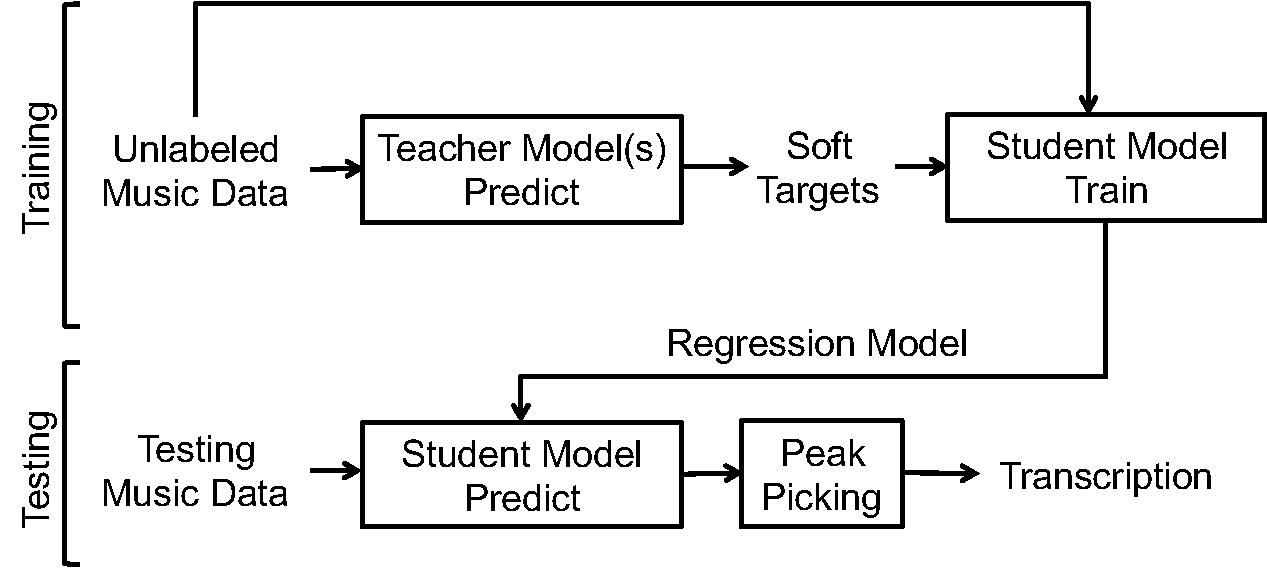
\includegraphics[width = 8 cm]{./figs/flowchart.pdf}
\caption{The flowchart of the proposed method}
\label{fig:flowchart}
\end{figure}

\subsection{Teacher Model}
The teacher model used in this paper is the drum transcription system presented by Wu and Lerch \cite{Wu2015a}. This NMF-based ADT system is chosen for its simplicity, its lack of need for substantial amounts of training data, as well as the adaptability in polyphonic mixtures; it extends the basic NMF model to Partially-Fixed Non-negative Matrix Factorization (PFNMF) by assuming the co-existence of both percussive and harmonic components in the audio signals. More specifically, the template matrix is split into a pre-defined part containing the drum templates which kept fixed and not iteratively updated and a randomly initialized part for modeling the remaining harmonic components in the signal. Formally, this can be expressed as $X \approx W_\mathrm{D}H_\mathrm{D} + W_\mathrm{H}H_\mathrm{H}$, with $X$ being a $m \times n$ magnitude spectrogram matrix with $m$ frequency bins and $n$ blocks, $W_\mathrm{D}$ and $W_\mathrm{H}$ representing the drum and harmonic dictionary matrices with a dimensionality of $m \times r_\mathrm{D}$ and $m \times r_\mathrm{H}$, and $H_\mathrm{D}$ and $H_\mathrm{H}$ their corresponding activation matrices with dimensionality of $r_\mathrm{D} \times n$ and $r_\mathrm{H} \times n$, respectively. $r_\mathrm{D}$ usually corresponds to the number of drums to detect (e.g., $r_\mathrm{D} = 3$ for the detection of HH, BD, and SD), and $r_\mathrm{H}$ is an user-defined parameter that varies according to the complexity of the target signal.  {\color{red}maybe you should mention somewhere that the implementation available online is used}

The basic flowchart of PFNMF is shown in \figref{fig:pfnmf}  {\color{red}I don't think you should reuse this plot from the paper.}. It firstly decomposes the magnitude spectrogram of the polyphonic mixtures with a fixed pre-trained drum dictionary $W_\mathrm{D}$ and a randomly initialized harmonic dictionary $W_\mathrm{H}$. Once the signal is decomposed, the NMF based activation function $H_\mathrm{D}(r, :)$ of each individual drum can be extracted, in which $r = \{1, 2, 3\}$ is the instrument index that corresponds to HH, BD, and SD, respectively. These activation functions can be interpreted as the activity level of each instrument over time, and a sharp peak indicates the presence of a single drum hit.

The conversion of the resulting activation functions into the soft targets takes another step of standard min-max scaling across the training data for each instrument; this process scales the soft targets to a numerical range between 0 and 1 and ensures the compatibility between the soft targets and the student model output (see Sect.~\ref{subsec:nn}). Finally, to introduce diversity into the soft targets, two PFNMF systems are created by initializing the algorithm with two different sets of drum dictionaries, forming an ensemble-like scenario that could potentially lead to better student performance. {\color{red}to waste some space: maybe some plot of activation functions comparing the different parametrization?}

\begin{figure}
\centering
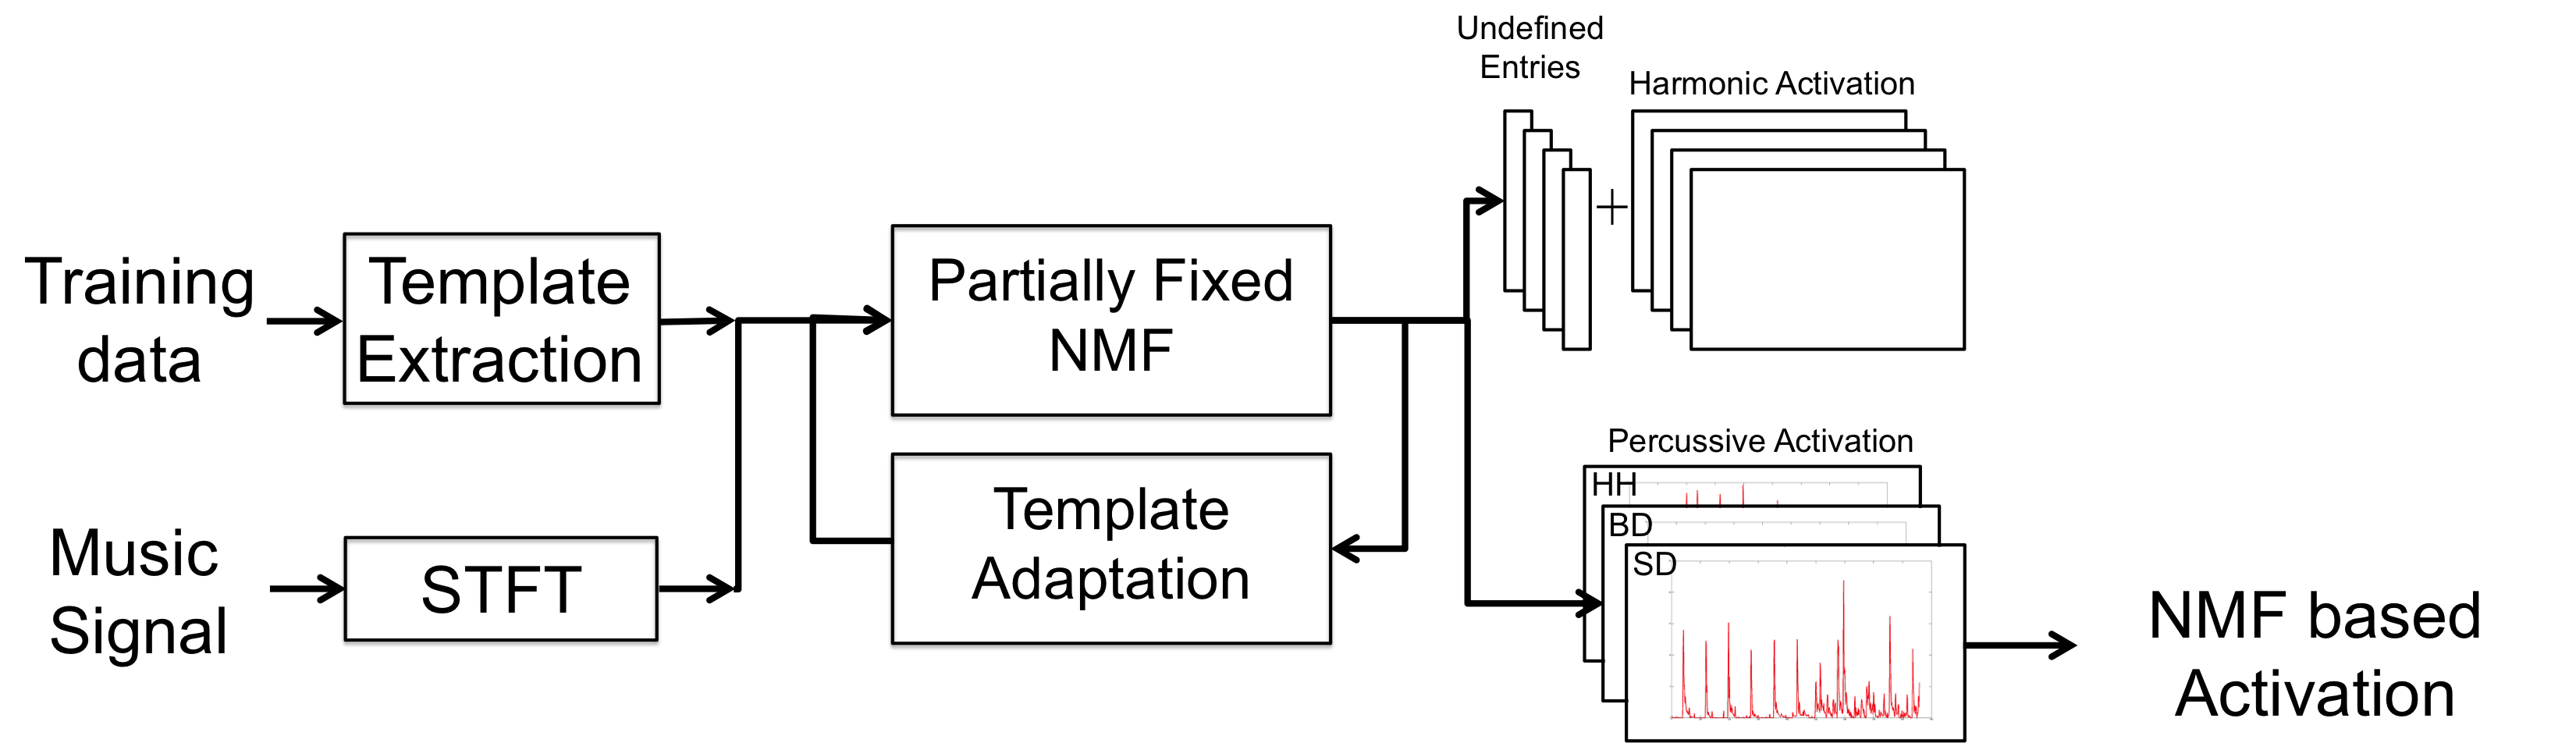
\includegraphics[width = 8 cm]{./figs/nmf.png}
\caption{The flowchart of PFNMF \cite{Wu2015a}}
\label{fig:pfnmf}
\end{figure}

\subsection{Student Model}\label{subsec:nn}
The proposed student model is a fully connected, feed-forward DNN with three hidden layers. A neural network is a graphic model that comprises multiple layers of interconnected non-linear units (i.e., neurons). The basic formulation of a neuron can be expressed in Eq.~(\ref{eq:nn_activ}), in which $a$ is the activation of the neuron, $W$ is the weight matrix, $b$ is the bias matrix, $l$ is the layer index, $j$ is the index of input neuron, and $k$ is the index of output neuron; $g( )$ is usually a non-linear function such as a \textit{sigmoid}, \textit{tanh} or \textit{relu}. When multiple layers of neurons are stacked, the model creates a complex non-linear transformation from the input to the output, which allows the model to approximate any arbitrary function with great flexibility. 

\begin{equation}\label{eq:nn_activ}
a_{k}^{l} = g\left( \sum_{j=1}^{M} W_{j} a_{j}^{l-1} + b_{j}^{l-1}\right)
\end{equation}

The architecture of the DNN in this paper is described as follows: the input layer contains $1025$ neurons that correspond to the size of the input representation. The first hidden layer comprises of a $1025$ neurons of \textit{tanh} activations with Batch Normalization {\color{red}since it's upper case, it implies a reference is missing}. The second and third hidden layers have $512$ and $32$ neurons with \textit{relu} activations, respectively. Finally, the output layer consists of 3 neurons with \textit{sigmoid} activations that represent the activities of three different drums (i.e., HH, SD, and BD). To solve the optimization problem of learning the weights $W$ in a DNN, a stochastic gradient descent based optimization method, $Adam$ {\color{red}why is this an equation? reference?}, is selected as the optimizer. The student neural network is configured as a regressor that minimizes the mean squared error between its output and the soft targets. A mini-batch consisting of $640$ blocks is used for training, and early stopping is applied when the minimum delta loss = $1e-6$ is not achieved for three consecutive epochs. {\color{red}rephrase the last sentence with the minimum loss? Confuses me a bit.}  {\color{red}wait: where have you introduced block and hop size and so on?} {\color{red}also: maybe it is too confusing to have activation functions as well as neural activations?}


\subsection{Implementation}
The input representation to both the teacher and student models is the magnitude spectrogram of the Short Time Fourier Transform (STFT) computed using a block size of 2048 and hop size of 512 samples with a Hann window applied to each block. Prior to the calculation of STFT, all of the audio signals are down-mixed to mono and resampled to a sampling rate of \unit[44.1]{kHz}. The resulting magnitude spectrogram is a $m \times n$ matrix, in which $m = 1025$ and $n = $ the number of blocks. 

For PFNMF, the authors' open source Matlab implementation\footnote{https://github.com/cwu307/NmfDrumToolbox} is used in our experiments. Since both the unlabeled music data and the testing data are polyphonic mixtures, the harmonic rank $r_\mathrm{H} $ for the PFNMF is set to $50$ as suggested in \cite{Wu2015a}. To speed up the process, template adaptation is deactivated. The extraction of the pre-defined (fixed) drum templates takes places on two publicly available drum datasets, namely the SMT-DRUM dataset \cite{Dittmar2014} and 200 drum machines \footnote{http://www.hexawe.net/mess/200.Drum.Machines}. Preliminary experiments show that these two sets of templates exhibit capabilities of capturing different types of drum sounds, bringing diversity into this learning paradigm. The construction of drum dictionary involves the concatenation of all the spectra and the extraction of the median spectrum for each individual instrument. It should be noted that, since the ENST drum dataset is the main test dataset for evaluation, no single drum hits from ENST are used for template extraction in order to ensure the generality of the proposed approach.

% deep learning toolboxes
% optimizer parameters = default
The DNN is implemented in Python using Keras\footnote{https://keras.io} with the Tensorflow\footnote{https://www.tensorflow.org} backend. The parameters of the optimizer are set to default. {\color{red}don't forget to add access dates to all links.}

% peak picking 
To get the final transcription results for evaluation, a standard peak picking method with a signal adaptive median threshold is used \cite{Lerch2012}. The median threshold $t(n)$ can be computed using Eq.~(\ref{eq:medianThres}), in which $\lambda$ is the offset coefficient relative to the maximum value, $p$ is the order (length) of the median filter, and the $n$ is the block index. All systems are using the same peak picking parameters of $p = $\unit[0.1]{s} and $\lambda = 0.12$ as described in \cite{Wu2015a}. No grid search is performed.  

\begin{equation}\label{eq:medianThres}
t(n) = \lambda * max(x) + median(x(n), p)
\end{equation} 

\section{Experiments}\label{sec:experiments}
\subsection{Dataset Description}
% unlabeled data
% criteria 
The collection of the unlabeled data is a crucial step for ensuring a successful learning process. Generally speaking, the unlabeled dataset should have following attributes: 
\begin{inparaenum}[(i)]
    \item   the collection should contain drums whenever possible,
    \item   the collection should be diverse in terms of music genres or playing styles,
    \item   the collection should contain no duplicates, and
    \item   the collection should be as consistent as possible in terms of audio quality. 
\end{inparaenum}
To build a collection that meets the above mentioned criteria, we compile a list from the Billboard Charts\footnote{http://www.billboard.com/charts Last accessed: 2017/04/25}. In particular, we start with an uniform distribution across a set of 4 genres selected for commonly featuring strong drum beats or rhythmic patterns, namely R\&B$\slash$HipHop, Pop, Rock, and Latin. For this study, 200 songs from each genre has been selected. All the songs are cross-checked for duplicates, and a final list of 800 songs has been compiled and retrieved from Youtube\footnote{https://www.youtube.com Last accessed: 2017/04/25} using open source Python library pafy\footnote{https://pypi.python.org/pypi/pafy Last accessed: 2017/04/25}. All songs are converted into mp3 files with a sampling rate of \unit[44.1]{kHz} using ffmepg\footnote{https://ffmpeg.org/download.html Last accessed: 2017/04/25}. The source code for constructing the unlabeled music dataset will be available in the Github repository\footnote{http:\\dummy.link}. In order to speed up the process while retaining the diversity, only a segment of 30 seconds from each song is used for training. Since the same unlabeled data is trained twice with two different sets of soft targets generated from two different teachers, the total duration of the training audio is \unit[800]{mins} (approximately \unit[13.5]{hours}), which is significantly larger than any of the existing drum labeled dataset. 

The most popular labeled drum dataset, ENST drum\cite{Gillet2006}, is used as the testing set for evaluation. This dataset consists of recordings from three different drummers performing on their own drum kits. The recordings from each drummer contain individual hits, short phrases of drum beats, drum solos, and short excerpts played with accompaniments. Since this paper focuses on ADT in polyphonic mixtures of music, only the \textit{minus one subset} is used for evaluation. This subset has 64 tracks of polyphonic music with a sampling rate of \unit[44.1]{kHz}. Each track in this subset has a length of approximately \unit[70]{s} with a variety of playing styles. More specifically, the subset contains various drum playing techniques such as ghost notes, flam, and drag, which is closer the real-world setting {\color{red}add your playing technique paper as reference?}. The accompaniments are mixed with their corresponding drum tracks using a scaling factor of 1/3 and 2/3 in order to be consistent with prior studies \cite{Paulus2009a, Wu2015a, Southall2016}. {\color{red}does the minus one set require indiviudal references or are these the same?}




\subsection{Experiment Setup}
The performance of the following systems is evaluated and compared: 
\begin{enumerate}[(i)]
\item   PFNMF (SMT): a PFNMF system initialized with a drum dictionary matrix extracted from SMT-DRUM dataset. This baseline system is used as a teacher model to generate the soft targets
\item   PFNMF (200D): a PFNMF system initialized with a drum dictionary matrix extracted from 200 drum machines dataset. This baseline system is the second teacher model for generating the soft targets
\item   PFNMF (SMT + 200D): another baseline system by simply taking the averaged activation functions of the above systems as the prediction output
\item   Linear SGD Regressor: a baseline student model using a simple linear regression with stochastic gradient descent optimization. A Python implementation of this method from the open source library, scikit-learn\footnote{http://scikit-learn.org Last accessed: 2017/04/25}, is used. All of the parameters are set to default.
\item   DNN: the proposed student model 
\end{enumerate}


\subsection{Metrics}
The evaluation metrics follow the standard calculation of the precision (P), recall (R), and F-measure (F). To be consistent with \cite{Gillet2008, Wu2015a, Southall2016}, an onset is considered to be a match with the ground truth if the time deviation between reference and detected onset time is less or equal to \unit[50]{ms}. It should be noted that some authors use more restrictive settings, compare, for instance, the \unit[30]{ms} and \unit[20]{ms} tolerance windows as used in \cite{Paulus2009a} and \cite{Vogl2017}, respectively.  

\subsection{Results}
The experiment results are shown in \tabref{tab:all_results}. The reported accuracies are the averaged F-measures across all 64 tracks from the ENST minus-one subset. Since the proposed method does not use the ENST drum dataset for training purposes, a three-fold cross validation scheme as reported in \cite{Paulus2009a, Wu2015a, Vogl2016, Vogl2017, Southall2016} is not necessary; this ensures the generality of the proposed method, but the comparison of the results with other systems might not be directly applicable.  {\color{red}I believe ISMIR requires a different table format --- maybe check?}
%
% ========== over all results
\begin{table*}
\centering
\begin{tabular}{ccccc|ccc}
\hline
\multicolumn{5}{c}{Experiments}                                                & \multicolumn{3}{c}{Averaged F-measure}           \\ \hline
\multicolumn{2}{c}{Role} & Method                  & Genres & \# Training Data & HH             & BD             & SD             \\ \hline
Teacher    & Baseline    & PFNMF (SMT)             & N/A    & N/A              & 0.685          & 0.8            & \textbf{0.501} \\
Teacher    & Baseline    & PFNMF (200D)       & N/A    & N/A              & 0.676          & 0.848          & 0.473          \\
           & Baseline    & PFNMF (SMT + 200D) & N/A    & N/A              & 0.686          & 0.828          & 0.474          \\
Student    & Baseline    & Linear SGD Regressor    & All    & 200 * 4 = 800    & 0.421          & 0.69           & 0.424          \\
Student    & Proposed    & DNN                     & All    & 200 * 4 = 800    & \textbf{0.772} & \textbf{0.851} & 0.443          \\ \hline
\end{tabular}
\caption{A comparison of the averaged F-measures between the proposed method and the baseline methods  {\color{red}why is there even a genres column in this table?}}
\label{tab:all_results}
\end{table*}
%
 {\color{red}I am not sure if reported 3 decimals is really helpful. I think it tempts to discuss differences that are no really there.}
The evaluation results show that both teacher systems PFNMF (SMT) and PFNMF (200D) perform similarly except for BD.  {\color{red}actually BD looks pretty similar to me!?} This could be due to the discrepancy of the pre-defined drum dictionaries. 
The 3rd simple baseline system PFNMF (SMT+200D) averaging the teacher outputs gives almost identical performance as the teacher systems. This result shows that a simple combination of the two teacher systems does not result in any improvement; thus, either the performance cannot be improved given the teacher information or a more sophisticated method is required for combining the outputs. 
The student baseline system is a simple linear regression model trained using the teacher-student learning paradigm as described in Sect.~\ref{sec:method}. This baseline serves as a sanity check for the necessity of a complex model such as DNN. As expected, the performance of the linear regression model is the worst among all the evaluated systems, indicating the need of deploying a non-linear model in order to benefit from this training scheme. 
Finally, the proposed DNN based student model is actually able to outperform both teachers with higher F-measures for both HH and BD. This result is generally encouraging and demonstrates the great potential of using unlabeled music data in ADT tasks. The results for the SD are somewhat inconclusive; here, one teacher actually outperforms all other systems.  {\color{red}sooooo, what are the possible reasons for that?}

Based on these results, another interesting question arises: does music genre play a role in the preparation of unlabeled data? To answer this question, another follow-up experiment has been conducted by training the proposed DNN model with unlabeled data of each individual genre. The experiment results are shown in \tabref{tab:genre_results}. In this experiment, the number of training samples is fixed at 200 in order to eliminate the influence of datasize. Interestingly, the best performance of different instruments, as highlighted in the table, belongs to different genres. This implies the advantage of having various genres in the training data, for they could potentially complement each other and boost the performance of the student model. 
{\color{red}BTW, should we add plots for all these results?}

Although the cross-genre model trained on the equally distributed data does not achieve the highest accuracy in each individual instrument, it is still better than majority of the single-genre models and generally well-balanced. The system trained on only Pop music seems to perform better than the model trained on all genres {\color{red}have you written this for different numbers? I don't see that. Also, is it really caomparable given the different number of training samples?}, however, the differences are marginal. Overall, maintaining a diverse unlabeled data in terms of music genre seems to be beneficial in this learning paradigm. {\color{red}any comment on WHY these different instruments work for specific genres?}
%
% ========= influence of genre
\begin{table*}
\centering
\begin{tabular}{cccccccc}
\hline
\multicolumn{5}{c}{Experiments}                               & \multicolumn{3}{c}{Averaged F-measure}           \\ \hline
\multicolumn{2}{c}{Role} & Method & Genres & \# Training Data & HH             & BD             & SD             \\ \hline
Student    &             & DNN    & Rock   & 200 * 1 = 200    & 0.755          & 0.828          & 0.432          \\
Student    &             & DNN    & Pop    & 200 * 1 = 200    & 0.771          & \textbf{0.846} & 0.446          \\
Student    &             & DNN    & RnB    & 200 * 1 = 200    & 0.733          & 0.830          & \textbf{0.474} \\
Student    &             & DNN    & Latin  & 200 * 1 = 200    & \textbf{0.772} & 0.828          & 0.439          \\
Student    & Proposed    & DNN    & All    & 50 * 4 = 200     & 0.765          & 0.841          & 0.441          \\ \hline
\end{tabular}
\caption{A comparison of different student models trained with unlabeled music data of different genres{\color{red}I don't understand what the last line of this table has anything to do with anything discussed? Or do you plan to add a paragraph about training set size? Then maybe do that in a separate table.}}
\label{tab:genre_results}
\end{table*}

From all of the above experiment results, HH shows the most clear and consistent improvement over the teacher models. This observation leads to another question: where do these improvements come from? A closer look at the experiment results reveals the strength of the DNN student model. As shown in \tabref{tab:pr_comp}, the DNN student model outperforms the teacher models on both precision and recall for HH. The DNN student model also achieves the highest BD precision. Since these improvements in precision are achieved without sacrificing recall, they might imply the reduction in false positives from the student model output. {\color{red}why don't we have the FP rate so we don't have to speculate?} One possible explanation is that the HH sounds in the unlabeled data has a higher agreement than the other instruments, and the student model is able to acquire a consistent internal representation of HH that leads to a more accurate estimation of the HH activation function during testing. {\color{red}Dude, you lost me there with the last sentence...}


%==== PRECISION OVER RECALL
\begin{table}
\begin{footnotesize}
\centering
\begin{tabular}{ccccccc}
\hline
\multirow{2}{*}{Method} & \multicolumn{2}{c}{HH}          & \multicolumn{2}{c}{BD}          & \multicolumn{2}{c}{SD}          \\ \cline{2-7} 
                        & P              & R              & P              & R              & P              & R              \\ \hline
PFNMF (SMT)             & 0.768          & 0.681          & 0.733          & \textbf{0.902} & \textbf{0.660} & \textbf{0.487} \\
PFNMF (200D)            & 0.748          & 0.676          & 0.818          & 0.893          & 0.591          & 0.486          \\
DNN                     & \textbf{0.868} & \textbf{0.718} & \textbf{0.827} & 0.888          & 0.592          & 0.434          \\ \hline
\end{tabular}
\caption{A comparison of precision (P) and recall (R) between student and teacher models}
\label{tab:pr_comp}
\end{footnotesize}
\end{table}


It is noticeable that the DNN student model seems to consistently struggle with SD. Since the SD tends to have larger spectral overlap with the other instruments, it is conceivable that DNN student model will have difficulties learning a robust internal representation for this instrument. A collection of unlabeled data with a stronger presence of snare drum might be possibly able to alleviate the problem, however, this issue requires further investigation before any conclusion can be drawn. In general, this deficiency in SD is also consistent with the previous studies \cite{Paulus2009a, Wu2015a, Southall2016, Vogl2016}, where the detection of snare drum in polyphonic mixtures has been reported as the most difficult task in ADT. {\color{red}Any insights to be gained from the linear regression getting results in the same range for SD?}

\section{Conclusion}\label{sec:conclusion}
This paper presented a system for Automatic Drum Transcription based on the teacher-student learning paradigm with the unlabeled music data. The proposed method integrates two NMF-based ADT teacher systems with a DNN-based student model by transferring knowledge using unlabeled music data, and the evaluation results indicate the possibility of obtaining a student model that outperforms the teacher model based on this approach. The experiment results also imply the benefit of having relevant music genres in the unlabeled dataset, which could lead to the construction of an improved unlabeled dataset in the future studies. The proposed method has the following advantages: first, the system has no prior knowledge of the testing data, which avoids over-fitting and suggests the generality of this approach. Second, the proposed method is able to support data-driven approaches with the need of large amounts of training data. Third, the proposed method could not only be easily applied to other ADT systems but also inform data-hungry systems from other transcription tasks or MIR problems in general.

The possible future directions of this work are:
\begin{inparaenum}[(i)]
    \item   Increasing the number and diversity of teacher systems. Since the proposed training scheme does not tie to any particular ADT approach, the teacher models can be easily swapped with other ADT expert systems. Intuitively, more teacher models should lead to a more versatile student model. However, the influence of having a more diverse pool of teacher systems still requires further investigation. 
    \item   Varying architectures and approaches of the student models. In addition to DNNs, other neural networks architecture may have great potential of achieving better student performance as well. For instance, the RNN based model that incorporates the temporal information could be a good fit in the context of ADT tasks. 
    \item   Evaluating different input representations. As reported by Cui et al.~\cite{Cui2017}, the student model is able to outperform the teacher model especially when it is trained on the same soft targets but with a stronger input representation. Following this observation, one possible future direction of this work is to investigate the effectiveness of other input representations such as CQT, Cepstrum, or Wavelet transforms. 
    \item   Evaluating alternative approaches for using unlabeled data. To fully benefit from the unlabeled data, it is also worth comparing the proposed method with other approaches such as unsupervised feature learning \cite{Raina2007a} in order to find the most effective strategy. 
\end{inparaenum}

The presented work represents only a preliminary study of what the authors see as a likely path for the future of training MIR systems as the issue of an insufficient amount of annotated data will only get worse with increasing complexity of machine learning systems applied to MIR tasks. Drawing on the vast potential of using existing state-of-the-art MIR-systems as teachers and the overwhelming public availability of unlabeled music data might enable new and exciting ways of creating new and more powerful MIR systems. {\color{red}Bah. Take the last paragraph or throw it away, I don't know...}  {\color{red}References: Read the guidelines in the paper template on abbreviations. Also, check the three bibtex warnings.}

% For bibtex users:
\bibliography{cw_ismir2017_drum}

\end{document}
